\documentclass[twoside]{book}

% Packages required by doxygen
\usepackage{fixltx2e}
\usepackage{calc}
\usepackage{doxygen}
\usepackage[export]{adjustbox} % also loads graphicx
\usepackage{graphicx}
\usepackage[utf8]{inputenc}
\usepackage{makeidx}
\usepackage{multicol}
\usepackage{multirow}
\PassOptionsToPackage{warn}{textcomp}
\usepackage{textcomp}
\usepackage[nointegrals]{wasysym}
\usepackage[table]{xcolor}

% Font selection
\usepackage[T1]{fontenc}
\usepackage[scaled=.90]{helvet}
\usepackage{courier}
\usepackage{amssymb}
\usepackage{sectsty}
\renewcommand{\familydefault}{\sfdefault}
\allsectionsfont{%
  \fontseries{bc}\selectfont%
  \color{darkgray}%
}
\renewcommand{\DoxyLabelFont}{%
  \fontseries{bc}\selectfont%
  \color{darkgray}%
}
\newcommand{\+}{\discretionary{\mbox{\scriptsize$\hookleftarrow$}}{}{}}

% Page & text layout
\usepackage{geometry}
\geometry{%
  a4paper,%
  top=2.5cm,%
  bottom=2.5cm,%
  left=2.5cm,%
  right=2.5cm%
}
\tolerance=750
\hfuzz=15pt
\hbadness=750
\setlength{\emergencystretch}{15pt}
\setlength{\parindent}{0cm}
\setlength{\parskip}{3ex plus 2ex minus 2ex}
\makeatletter
\renewcommand{\paragraph}{%
  \@startsection{paragraph}{4}{0ex}{-1.0ex}{1.0ex}{%
    \normalfont\normalsize\bfseries\SS@parafont%
  }%
}
\renewcommand{\subparagraph}{%
  \@startsection{subparagraph}{5}{0ex}{-1.0ex}{1.0ex}{%
    \normalfont\normalsize\bfseries\SS@subparafont%
  }%
}
\makeatother

% Headers & footers
\usepackage{fancyhdr}
\pagestyle{fancyplain}
\fancyhead[LE]{\fancyplain{}{\bfseries\thepage}}
\fancyhead[CE]{\fancyplain{}{}}
\fancyhead[RE]{\fancyplain{}{\bfseries\leftmark}}
\fancyhead[LO]{\fancyplain{}{\bfseries\rightmark}}
\fancyhead[CO]{\fancyplain{}{}}
\fancyhead[RO]{\fancyplain{}{\bfseries\thepage}}
\fancyfoot[LE]{\fancyplain{}{}}
\fancyfoot[CE]{\fancyplain{}{}}
\fancyfoot[RE]{\fancyplain{}{\bfseries\scriptsize Generated by Doxygen }}
\fancyfoot[LO]{\fancyplain{}{\bfseries\scriptsize Generated by Doxygen }}
\fancyfoot[CO]{\fancyplain{}{}}
\fancyfoot[RO]{\fancyplain{}{}}
\renewcommand{\footrulewidth}{0.4pt}
\renewcommand{\chaptermark}[1]{%
  \markboth{#1}{}%
}
\renewcommand{\sectionmark}[1]{%
  \markright{\thesection\ #1}%
}

% Indices & bibliography
\usepackage{natbib}
\usepackage[titles]{tocloft}
\setcounter{tocdepth}{3}
\setcounter{secnumdepth}{5}
\makeindex

% Hyperlinks (required, but should be loaded last)
\usepackage{ifpdf}
\ifpdf
  \usepackage[pdftex,pagebackref=true]{hyperref}
\else
  \usepackage[ps2pdf,pagebackref=true]{hyperref}
\fi
\hypersetup{%
  colorlinks=true,%
  linkcolor=blue,%
  citecolor=blue,%
  unicode%
}

% Custom commands
\newcommand{\clearemptydoublepage}{%
  \newpage{\pagestyle{empty}\cleardoublepage}%
}

\usepackage{caption}
\captionsetup{labelsep=space,justification=centering,font={bf},singlelinecheck=off,skip=4pt,position=top}

%===== C O N T E N T S =====

\begin{document}

% Titlepage & ToC
\hypersetup{pageanchor=false,
             bookmarksnumbered=true,
             pdfencoding=unicode
            }
\pagenumbering{alph}
\begin{titlepage}
\vspace*{7cm}
\begin{center}%
{\Large My Project }\\
\vspace*{1cm}
{\large Generated by Doxygen 1.8.14}\\
\end{center}
\end{titlepage}
\clearemptydoublepage
\pagenumbering{roman}
\tableofcontents
\clearemptydoublepage
\pagenumbering{arabic}
\hypersetup{pageanchor=true}

%--- Begin generated contents ---
\chapter{Hierarchical Index}
\section{Class Hierarchy}
This inheritance list is sorted roughly, but not completely, alphabetically\+:\begin{DoxyCompactList}
\item \contentsline{section}{Button\+Listener}{\pageref{class_button_listener}}{}
\begin{DoxyCompactList}
\item \contentsline{section}{Shoot\+Control}{\pageref{class_shoot_control}}{}
\end{DoxyCompactList}
\item \contentsline{section}{ir\+\_\+msg}{\pageref{structir__msg}}{}
\item \contentsline{section}{I\+R\+Control}{\pageref{class_i_r_control}}{}
\begin{DoxyCompactList}
\item \contentsline{section}{Shoot\+Control}{\pageref{class_shoot_control}}{}
\end{DoxyCompactList}
\item \contentsline{section}{msg\+\_\+listener}{\pageref{classmsg__listener}}{}
\begin{DoxyCompactList}
\item \contentsline{section}{msg\+\_\+logger}{\pageref{classmsg__logger}}{}
\end{DoxyCompactList}
\item \contentsline{section}{pause\+\_\+listener}{\pageref{classpause__listener}}{}
\begin{DoxyCompactList}
\item \contentsline{section}{msg\+\_\+decoder}{\pageref{classmsg__decoder}}{}
\end{DoxyCompactList}
\item task\begin{DoxyCompactList}
\item \contentsline{section}{Button}{\pageref{class_button}}{}
\item \contentsline{section}{msg\+\_\+decoder}{\pageref{classmsg__decoder}}{}
\item \contentsline{section}{msg\+\_\+logger}{\pageref{classmsg__logger}}{}
\item \contentsline{section}{pause\+\_\+detector}{\pageref{classpause__detector}}{}
\item \contentsline{section}{Shoot\+Control}{\pageref{class_shoot_control}}{}
\end{DoxyCompactList}
\end{DoxyCompactList}

\chapter{Class Index}
\section{Class List}
Here are the classes, structs, unions and interfaces with brief descriptions\+:\begin{DoxyCompactList}
\item\contentsline{section}{\mbox{\hyperlink{class_button}{Button}} \\*This class is used to make a button object }{\pageref{class_button}}{}
\item\contentsline{section}{\mbox{\hyperlink{class_button_listener}{Button\+Listener}} \\*A class containing the virtual button\+Pressed function }{\pageref{class_button_listener}}{}
\item\contentsline{section}{\mbox{\hyperlink{class_buzzer_control}{Buzzer\+Control}} \\*This class is used to control the buzzer }{\pageref{class_buzzer_control}}{}
\item\contentsline{section}{\mbox{\hyperlink{class_display_control}{Display\+Control}} \\*This class is used to show the command value on the screen }{\pageref{class_display_control}}{}
\item\contentsline{section}{\mbox{\hyperlink{class_game_leader}{Game\+Leader}} \\*This class is used to make the game }{\pageref{class_game_leader}}{}
\item\contentsline{section}{\mbox{\hyperlink{class_game_logs}{Game\+Logs}} \\*This class is used to track all the hits during the game and to print them at the end }{\pageref{class_game_logs}}{}
\item\contentsline{section}{\mbox{\hyperlink{structir__msg}{ir\+\_\+msg}} \\*This struct gets used to split the message in two parts }{\pageref{structir__msg}}{}
\item\contentsline{section}{\mbox{\hyperlink{class_i_r_control}{I\+R\+Control}} \\*This class is used to control the IR signal }{\pageref{class_i_r_control}}{}
\item\contentsline{section}{\mbox{\hyperlink{class_keypad}{Keypad}} \\*In this class you can find the pin setup and initialize the characters }{\pageref{class_keypad}}{}
\item\contentsline{section}{\mbox{\hyperlink{class_keypad_control}{Keypad\+Control}} \\*This class is used to control the keypad }{\pageref{class_keypad_control}}{}
\item\contentsline{section}{\mbox{\hyperlink{classmsg__decoder}{msg\+\_\+decoder}} }{\pageref{classmsg__decoder}}{}
\item\contentsline{section}{\mbox{\hyperlink{classmsg__listener}{msg\+\_\+listener}} }{\pageref{classmsg__listener}}{}
\item\contentsline{section}{\mbox{\hyperlink{classmsg__logger}{msg\+\_\+logger}} }{\pageref{classmsg__logger}}{}
\item\contentsline{section}{\mbox{\hyperlink{class_msg_decoder}{Msg\+Decoder}} \\*This class decodes the incoming message and sends it to another class }{\pageref{class_msg_decoder}}{}
\item\contentsline{section}{\mbox{\hyperlink{class_msg_listener}{Msg\+Listener}} \\*This class constains the virtual msg\+Received function }{\pageref{class_msg_listener}}{}
\item\contentsline{section}{\mbox{\hyperlink{classpause__detector}{pause\+\_\+detector}} }{\pageref{classpause__detector}}{}
\item\contentsline{section}{\mbox{\hyperlink{classpause__listener}{pause\+\_\+listener}} }{\pageref{classpause__listener}}{}
\item\contentsline{section}{\mbox{\hyperlink{class_pause_detector}{Pause\+Detector}} \\*This class detects the pauses in a IR signal and sends them to another class }{\pageref{class_pause_detector}}{}
\item\contentsline{section}{\mbox{\hyperlink{class_pause_listener}{Pause\+Listener}} \\*This class contains the virtual function pause\+Detected }{\pageref{class_pause_listener}}{}
\item\contentsline{section}{\mbox{\hyperlink{class_player_control}{Player\+Control}} \\*This class controls the player tasks }{\pageref{class_player_control}}{}
\item\contentsline{section}{\mbox{\hyperlink{class_player_data}{Player\+Data}} \\*This class contains all the playerdata }{\pageref{class_player_data}}{}
\item\contentsline{section}{\mbox{\hyperlink{class_send_control}{Send\+Control}} \\*This class is used to send the data }{\pageref{class_send_control}}{}
\item\contentsline{section}{\mbox{\hyperlink{class_shoot_control}{Shoot\+Control}} \\*This class encodes and sends the message to be sent to the \mbox{\hyperlink{class_i_r_control}{I\+R\+Control}} class and controls the laser }{\pageref{class_shoot_control}}{}
\item\contentsline{section}{\mbox{\hyperlink{class_weapon}{Weapon}} \\*This class contains the data of the weapon }{\pageref{class_weapon}}{}
\end{DoxyCompactList}

\chapter{Class Documentation}
\hypertarget{class_button}{}\section{Button Class Reference}
\label{class_button}\index{Button@{Button}}


This class is used to make a button object.  




{\ttfamily \#include $<$Button.\+hpp$>$}

Inheritance diagram for Button\+:\begin{figure}[H]
\begin{center}
\leavevmode
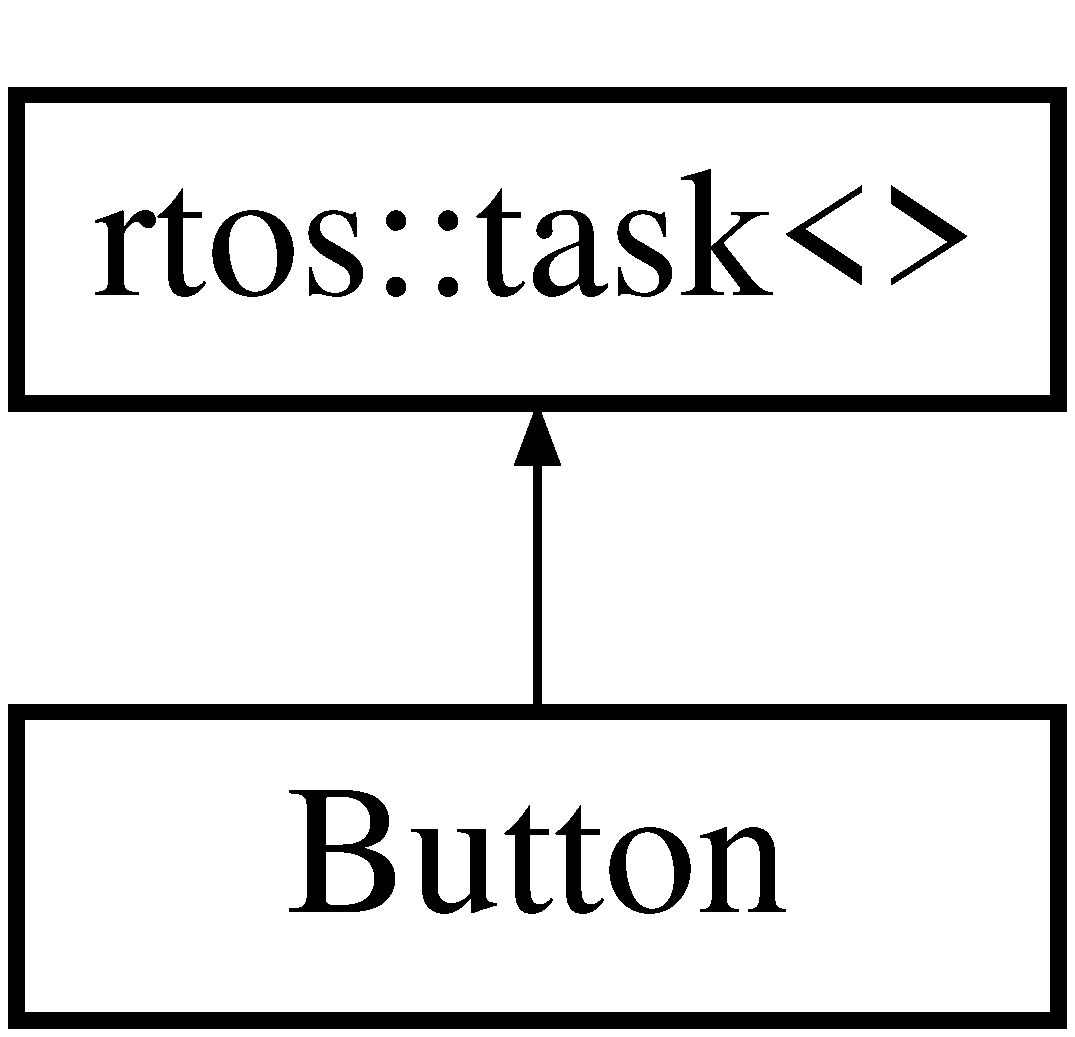
\includegraphics[height=2.000000cm]{class_button}
\end{center}
\end{figure}
\subsection*{Public Member Functions}
\begin{DoxyCompactItemize}
\item 
\mbox{\hyperlink{class_button_a7771486e8e6649ee30c85ab5580796da}{Button}} (const char $\ast$name, int priority, hwlib\+::pin\+\_\+in \&pin\+\_\+button, \mbox{\hyperlink{class_button_listener}{Button\+Listener}} \&listener, unsigned int buttonnumber)
\begin{DoxyCompactList}\small\item\em This is the constructor for a button. \end{DoxyCompactList}\item 
void \mbox{\hyperlink{class_button_a4cc671cc425acd0ee1b8f2f437cf40db}{main}} () override
\begin{DoxyCompactList}\small\item\em The main contains the state machine. \end{DoxyCompactList}\end{DoxyCompactItemize}


\subsection{Detailed Description}
This class is used to make a button object. 

\subsection{Constructor \& Destructor Documentation}
\mbox{\Hypertarget{class_button_a7771486e8e6649ee30c85ab5580796da}\label{class_button_a7771486e8e6649ee30c85ab5580796da}} 
\index{Button@{Button}!Button@{Button}}
\index{Button@{Button}!Button@{Button}}
\subsubsection{\texorpdfstring{Button()}{Button()}}
{\footnotesize\ttfamily Button\+::\+Button (\begin{DoxyParamCaption}\item[{const char $\ast$}]{name,  }\item[{int}]{priority,  }\item[{hwlib\+::pin\+\_\+in \&}]{pin\+\_\+button,  }\item[{\mbox{\hyperlink{class_button_listener}{Button\+Listener}} \&}]{listener,  }\item[{unsigned int}]{buttonnumber }\end{DoxyParamCaption})\hspace{0.3cm}{\ttfamily [inline]}}



This is the constructor for a button. 

The constructor expects a listener which is the class that owns the button. 

\subsection{Member Function Documentation}
\mbox{\Hypertarget{class_button_a4cc671cc425acd0ee1b8f2f437cf40db}\label{class_button_a4cc671cc425acd0ee1b8f2f437cf40db}} 
\index{Button@{Button}!main@{main}}
\index{main@{main}!Button@{Button}}
\subsubsection{\texorpdfstring{main()}{main()}}
{\footnotesize\ttfamily void Button\+::main (\begin{DoxyParamCaption}{ }\end{DoxyParamCaption})\hspace{0.3cm}{\ttfamily [inline]}, {\ttfamily [override]}}



The main contains the state machine. 

The main only consists of one state the wait\+\_\+for\+\_\+button\+\_\+press state. The state waits for a clock that gets called every 100 ms. When the clock is called the button pin gets checked for input. If there is a input the function buttonpressed in the listener gets called. 

The documentation for this class was generated from the following file\+:\begin{DoxyCompactItemize}
\item 
C\+:/ti-\/software/thema\+\_\+opdracht\+\_\+lasergame/\+Player/\mbox{\hyperlink{_button_8hpp}{Button.\+hpp}}\end{DoxyCompactItemize}

\hypertarget{class_button_listener}{}\section{Button\+Listener Class Reference}
\label{class_button_listener}\index{Button\+Listener@{Button\+Listener}}


A class containing the virtual button\+Pressed function.  




{\ttfamily \#include $<$Button\+Listener.\+hpp$>$}

Inheritance diagram for Button\+Listener\+:\begin{figure}[H]
\begin{center}
\leavevmode
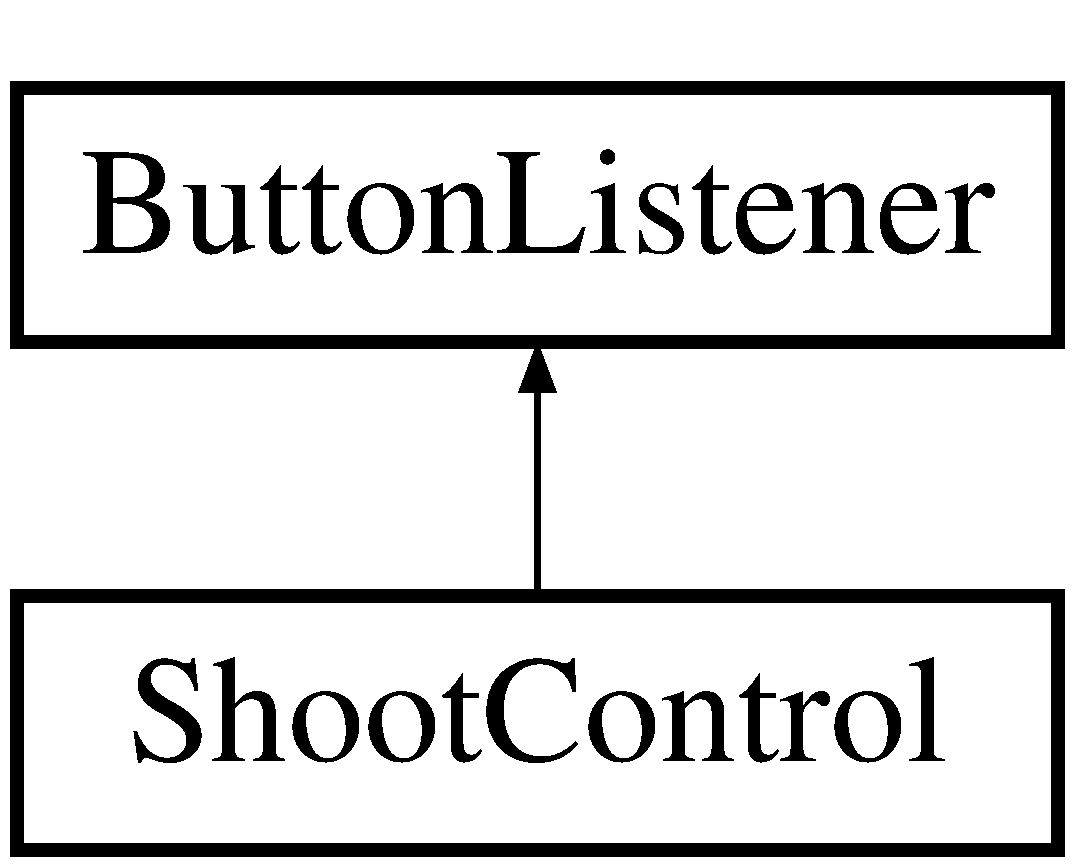
\includegraphics[height=2.000000cm]{class_button_listener}
\end{center}
\end{figure}
\subsection*{Public Member Functions}
\begin{DoxyCompactItemize}
\item 
\mbox{\Hypertarget{class_button_listener_a444f84514e359443020463edc129cd12}\label{class_button_listener_a444f84514e359443020463edc129cd12}} 
virtual void {\bfseries button\+Detected} ()=0
\item 
\mbox{\Hypertarget{class_button_listener_a669be11c0665a02e9501ee4ca03d8a8d}\label{class_button_listener_a669be11c0665a02e9501ee4ca03d8a8d}} 
virtual void \mbox{\hyperlink{class_button_listener_a669be11c0665a02e9501ee4ca03d8a8d}{button\+Pressed}} (unsigned int \&buttonnumber)=0
\begin{DoxyCompactList}\small\item\em This virtual function gets called by a button and gets overwritten in another class. \end{DoxyCompactList}\end{DoxyCompactItemize}


\subsection{Detailed Description}
A class containing the virtual button\+Pressed function. 

The documentation for this class was generated from the following files\+:\begin{DoxyCompactItemize}
\item 
C\+:/ti-\/software/thema\+\_\+opdracht\+\_\+lasergame/\+I\+R\+\_\+send/button\+\_\+listener.\+hpp\item 
C\+:/ti-\/software/thema\+\_\+opdracht\+\_\+lasergame/\+Player/\mbox{\hyperlink{_button_listener_8hpp}{Button\+Listener.\+hpp}}\end{DoxyCompactItemize}

\hypertarget{structir__msg}{}\section{ir\+\_\+msg Struct Reference}
\label{structir__msg}\index{ir\+\_\+msg@{ir\+\_\+msg}}


This struct gets used to split the message in two parts.  




{\ttfamily \#include $<$Msg\+Listener.\+hpp$>$}

\subsection*{Public Attributes}
\begin{DoxyCompactItemize}
\item 
\mbox{\Hypertarget{structir__msg_a1aba19ec600f05dbf3e20cd94585f2b7}\label{structir__msg_a1aba19ec600f05dbf3e20cd94585f2b7}} 
uint8\+\_\+t {\bfseries player}
\item 
\mbox{\Hypertarget{structir__msg_a186ea1a98c46be88a9664b2ca285566f}\label{structir__msg_a186ea1a98c46be88a9664b2ca285566f}} 
uint8\+\_\+t {\bfseries data}
\end{DoxyCompactItemize}


\subsection{Detailed Description}
This struct gets used to split the message in two parts. 

The message gets split into the player part and the data part. 

The documentation for this struct was generated from the following file\+:\begin{DoxyCompactItemize}
\item 
C\+:/ti-\/software/thema\+\_\+opdracht\+\_\+lasergame/\+Player/\mbox{\hyperlink{_msg_listener_8hpp}{Msg\+Listener.\+hpp}}\end{DoxyCompactItemize}

\hypertarget{class_i_r_control}{}\section{I\+R\+Control Class Reference}
\label{class_i_r_control}\index{I\+R\+Control@{I\+R\+Control}}
Inheritance diagram for I\+R\+Control\+:\begin{figure}[H]
\begin{center}
\leavevmode
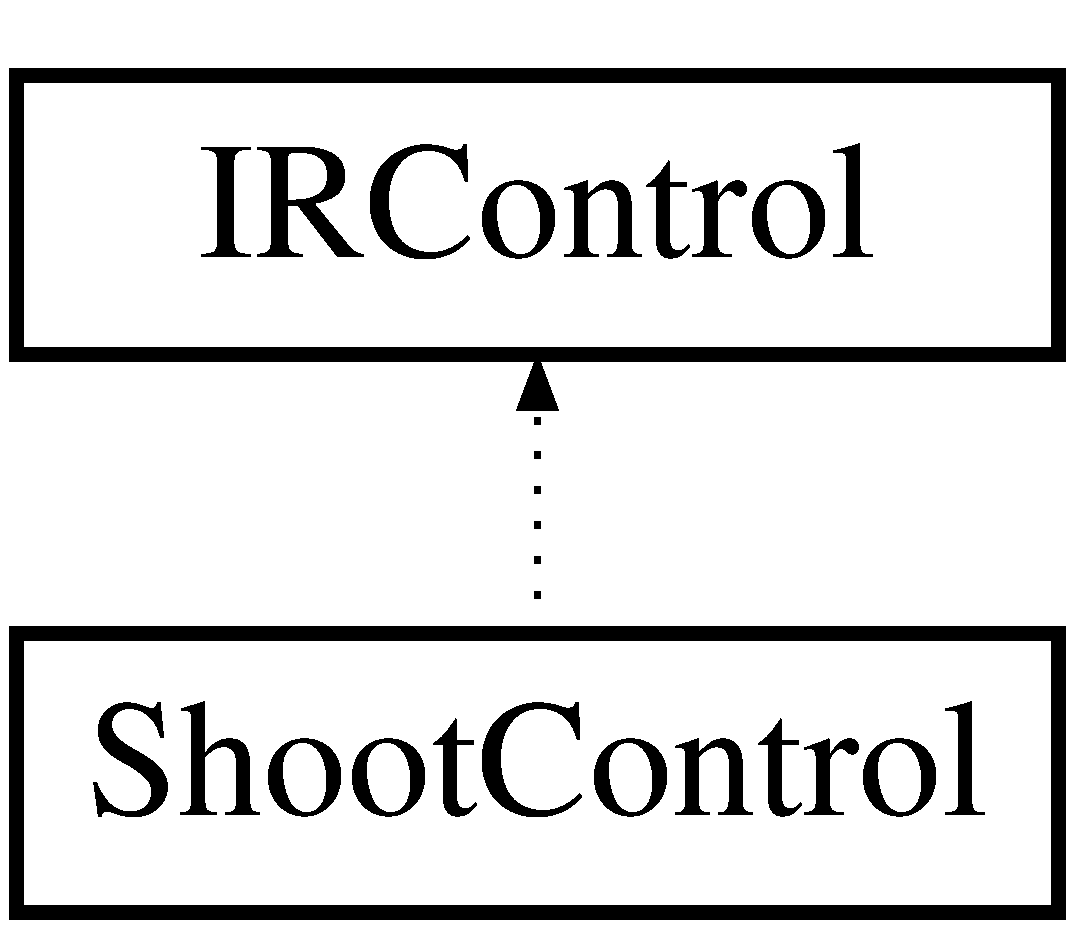
\includegraphics[height=2.000000cm]{class_i_r_control}
\end{center}
\end{figure}
\subsection*{Public Member Functions}
\begin{DoxyCompactItemize}
\item 
\mbox{\Hypertarget{class_i_r_control_ac16a197b453b4bd18874dbc1ef2d3cf4}\label{class_i_r_control_ac16a197b453b4bd18874dbc1ef2d3cf4}} 
void {\bfseries send} (const uint16\+\_\+t \&data)
\item 
\mbox{\Hypertarget{class_i_r_control_a12e0082a899fc811fa70c5cbe59e18d0}\label{class_i_r_control_a12e0082a899fc811fa70c5cbe59e18d0}} 
void {\bfseries pulse} (bool data)
\end{DoxyCompactItemize}


The documentation for this class was generated from the following file\+:\begin{DoxyCompactItemize}
\item 
C\+:/ti-\/software/thema\+\_\+opdracht\+\_\+lasergame/\+I\+R\+\_\+send/I\+R\+Control.\+hpp\end{DoxyCompactItemize}

\hypertarget{classmsg__decoder}{}\section{msg\+\_\+decoder Class Reference}
\label{classmsg__decoder}\index{msg\+\_\+decoder@{msg\+\_\+decoder}}
Inheritance diagram for msg\+\_\+decoder\+:\begin{figure}[H]
\begin{center}
\leavevmode
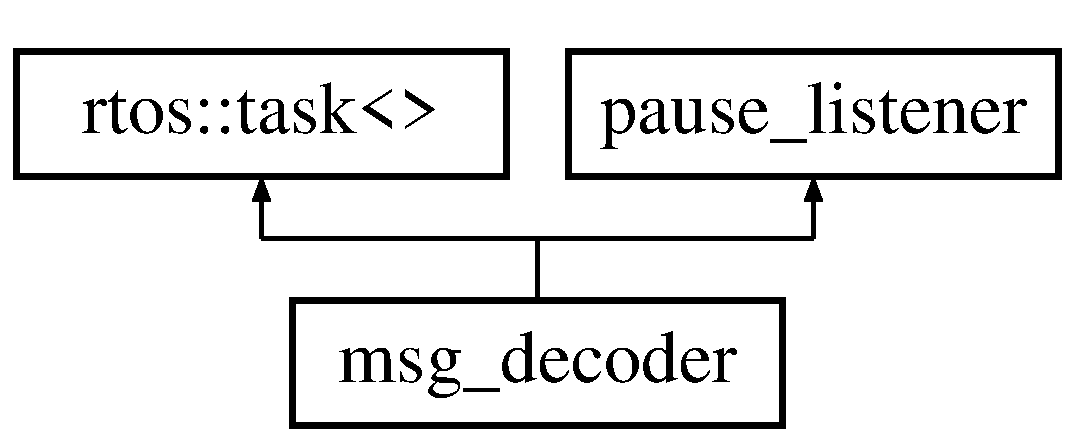
\includegraphics[height=2.000000cm]{classmsg__decoder}
\end{center}
\end{figure}
\subsection*{Public Member Functions}
\begin{DoxyCompactItemize}
\item 
\mbox{\Hypertarget{classmsg__decoder_ae9b18eff0ca3fc3d3c9248e4e38fd246}\label{classmsg__decoder_ae9b18eff0ca3fc3d3c9248e4e38fd246}} 
{\bfseries msg\+\_\+decoder} (const char $\ast$name, \mbox{\hyperlink{classmsg__listener}{msg\+\_\+listener}} \&listener)
\item 
\mbox{\Hypertarget{classmsg__decoder_a990f6ed2f479d61c8fbd0ceeba80a165}\label{classmsg__decoder_a990f6ed2f479d61c8fbd0ceeba80a165}} 
virtual void {\bfseries pause\+\_\+detected} (int pause\+\_\+length) override
\item 
\mbox{\Hypertarget{classmsg__decoder_a346301483ec894f687c93227d09a00a6}\label{classmsg__decoder_a346301483ec894f687c93227d09a00a6}} 
void {\bfseries print\+Byte} (uint8\+\_\+t byte)
\item 
\mbox{\Hypertarget{classmsg__decoder_af25ea64b8c252a82e879451c1fce6d24}\label{classmsg__decoder_af25ea64b8c252a82e879451c1fce6d24}} 
void {\bfseries print\+Bytes} (uint16\+\_\+t byte)
\item 
\mbox{\Hypertarget{classmsg__decoder_a17ed2804e6ec965a054b53e54b257d30}\label{classmsg__decoder_a17ed2804e6ec965a054b53e54b257d30}} 
bool {\bfseries check} (unsigned int m)
\item 
\mbox{\Hypertarget{classmsg__decoder_a8954f1ed668d0428ab4191ba6013c659}\label{classmsg__decoder_a8954f1ed668d0428ab4191ba6013c659}} 
void {\bfseries main} () override
\end{DoxyCompactItemize}


The documentation for this class was generated from the following file\+:\begin{DoxyCompactItemize}
\item 
C\+:/ti-\/software/thema\+\_\+opdracht\+\_\+lasergame/\+I\+R\+\_\+receive/msg\+\_\+decoder.\+hpp\end{DoxyCompactItemize}

\hypertarget{classmsg__listener}{}\section{msg\+\_\+listener Class Reference}
\label{classmsg__listener}\index{msg\+\_\+listener@{msg\+\_\+listener}}
Inheritance diagram for msg\+\_\+listener\+:\begin{figure}[H]
\begin{center}
\leavevmode
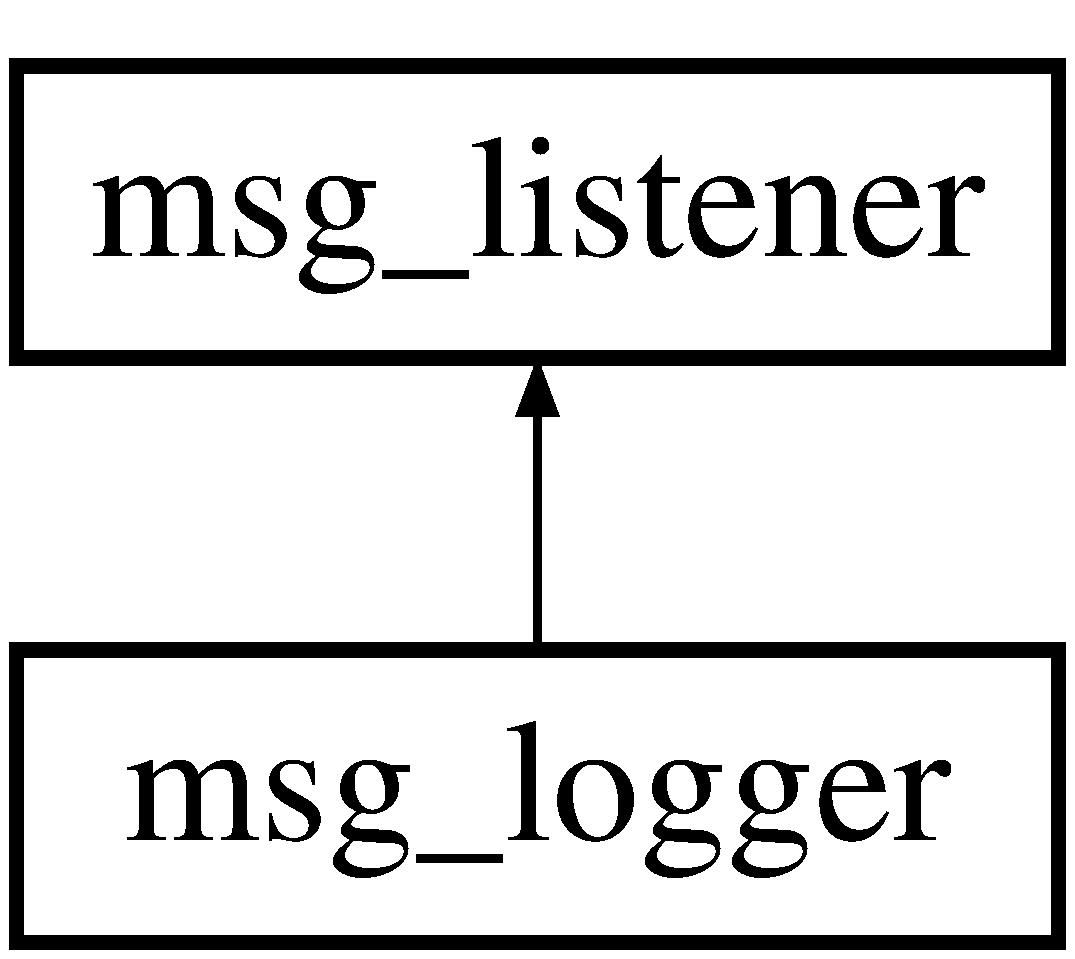
\includegraphics[height=2.000000cm]{classmsg__listener}
\end{center}
\end{figure}
\subsection*{Public Member Functions}
\begin{DoxyCompactItemize}
\item 
\mbox{\Hypertarget{classmsg__listener_ab82f5182543d7e9f2579e5d6f47cc3b9}\label{classmsg__listener_ab82f5182543d7e9f2579e5d6f47cc3b9}} 
virtual void {\bfseries msg\+\_\+received} (const \mbox{\hyperlink{structir__msg}{ir\+\_\+msg}} \&msg)=0
\end{DoxyCompactItemize}


The documentation for this class was generated from the following file\+:\begin{DoxyCompactItemize}
\item 
C\+:/ti-\/software/thema\+\_\+opdracht\+\_\+lasergame/\+I\+R\+\_\+receive/msg\+\_\+listener.\+hpp\end{DoxyCompactItemize}

\hypertarget{classmsg__logger}{}\section{msg\+\_\+logger Class Reference}
\label{classmsg__logger}\index{msg\+\_\+logger@{msg\+\_\+logger}}
Inheritance diagram for msg\+\_\+logger\+:\begin{figure}[H]
\begin{center}
\leavevmode
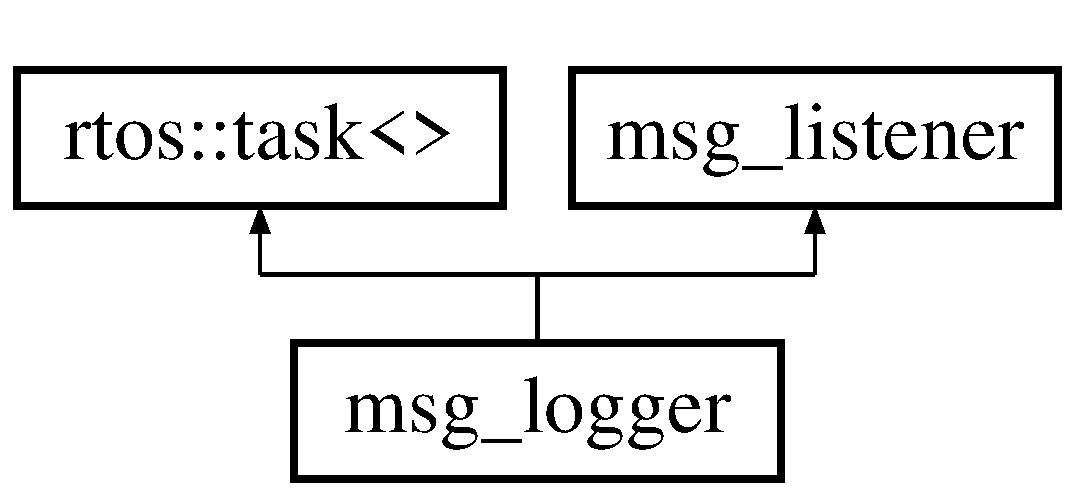
\includegraphics[height=2.000000cm]{classmsg__logger}
\end{center}
\end{figure}
\subsection*{Public Member Functions}
\begin{DoxyCompactItemize}
\item 
\mbox{\Hypertarget{classmsg__logger_a3ae26749c728559cb363631a7810f014}\label{classmsg__logger_a3ae26749c728559cb363631a7810f014}} 
{\bfseries msg\+\_\+logger} (const char $\ast$name)
\item 
\mbox{\Hypertarget{classmsg__logger_a1d6398b619717cccc6e125a660d6ad30}\label{classmsg__logger_a1d6398b619717cccc6e125a660d6ad30}} 
virtual void {\bfseries msg\+\_\+received} (const \mbox{\hyperlink{structir__msg}{ir\+\_\+msg}} \&msg) override
\item 
\mbox{\Hypertarget{classmsg__logger_ac674c87e969c7a22f483c809bf868460}\label{classmsg__logger_ac674c87e969c7a22f483c809bf868460}} 
void {\bfseries main} () override
\end{DoxyCompactItemize}


The documentation for this class was generated from the following file\+:\begin{DoxyCompactItemize}
\item 
C\+:/ti-\/software/thema\+\_\+opdracht\+\_\+lasergame/\+I\+R\+\_\+receive/msg\+\_\+logger.\+hpp\end{DoxyCompactItemize}

\hypertarget{classpause__detector}{}\section{pause\+\_\+detector Class Reference}
\label{classpause__detector}\index{pause\+\_\+detector@{pause\+\_\+detector}}
Inheritance diagram for pause\+\_\+detector\+:\begin{figure}[H]
\begin{center}
\leavevmode
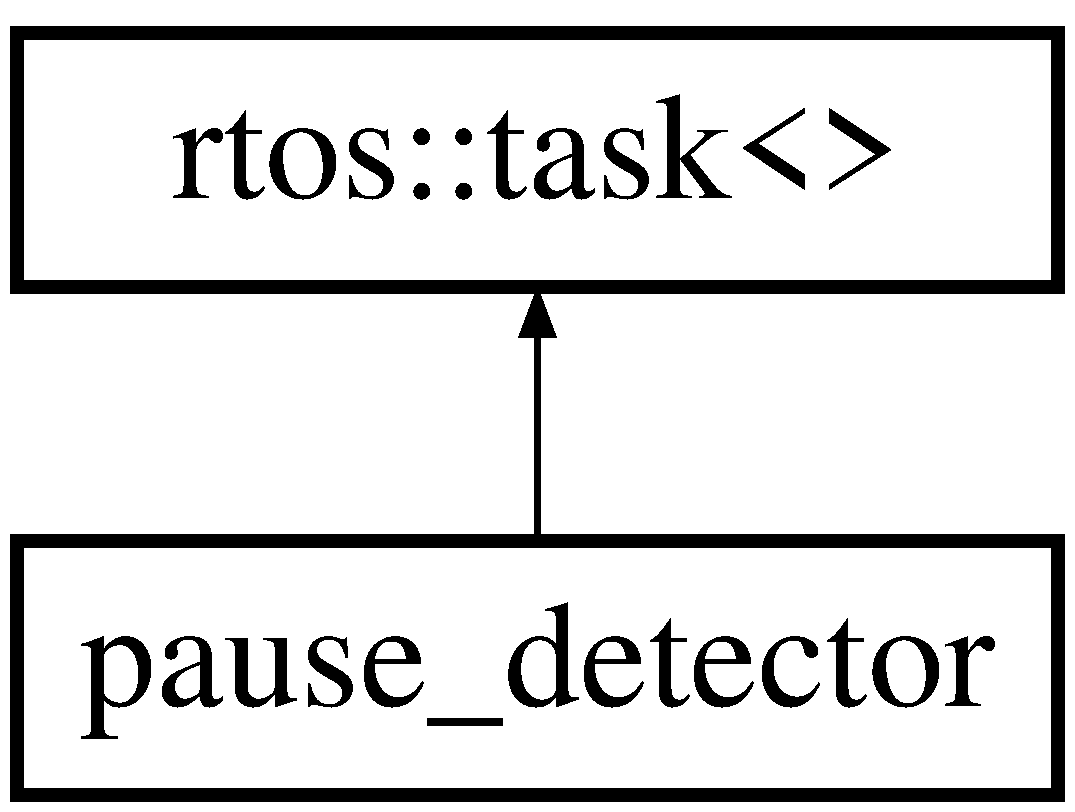
\includegraphics[height=2.000000cm]{classpause__detector}
\end{center}
\end{figure}
\subsection*{Public Member Functions}
\begin{DoxyCompactItemize}
\item 
\mbox{\Hypertarget{classpause__detector_a86b2fb4fd1032eb81517bc27ee9f6f2e}\label{classpause__detector_a86b2fb4fd1032eb81517bc27ee9f6f2e}} 
{\bfseries pause\+\_\+detector} (const char $\ast$name, hwlib\+::pin\+\_\+in \&irp, \mbox{\hyperlink{classpause__listener}{pause\+\_\+listener}} \&listener)
\item 
\mbox{\Hypertarget{classpause__detector_ac2d43c7fd2489b622359de11bfdc1cc2}\label{classpause__detector_ac2d43c7fd2489b622359de11bfdc1cc2}} 
void {\bfseries main} () override
\end{DoxyCompactItemize}


The documentation for this class was generated from the following file\+:\begin{DoxyCompactItemize}
\item 
C\+:/ti-\/software/thema\+\_\+opdracht\+\_\+lasergame/\+I\+R\+\_\+receive/pause\+\_\+detector.\+hpp\end{DoxyCompactItemize}

\hypertarget{classpause__listener}{}\section{pause\+\_\+listener Class Reference}
\label{classpause__listener}\index{pause\+\_\+listener@{pause\+\_\+listener}}
Inheritance diagram for pause\+\_\+listener\+:\begin{figure}[H]
\begin{center}
\leavevmode
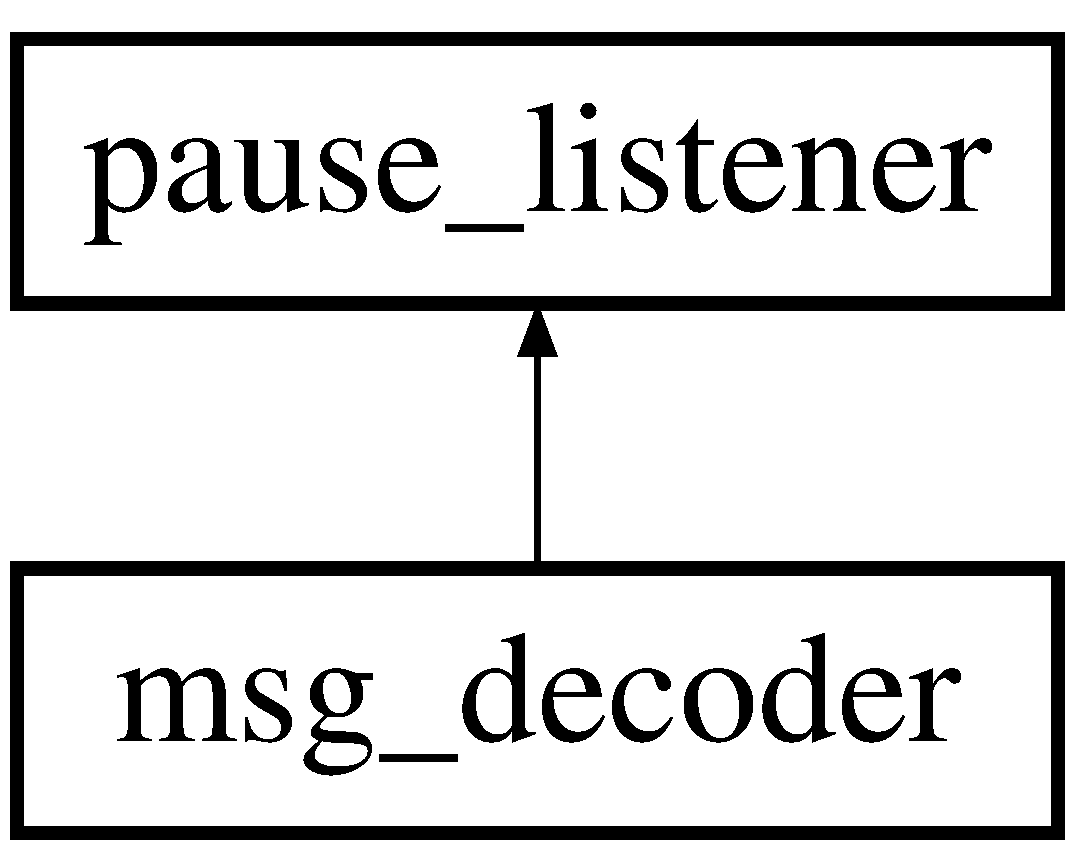
\includegraphics[height=2.000000cm]{classpause__listener}
\end{center}
\end{figure}
\subsection*{Public Member Functions}
\begin{DoxyCompactItemize}
\item 
\mbox{\Hypertarget{classpause__listener_a8c028680b7e4b26b7258417e0fb4cfca}\label{classpause__listener_a8c028680b7e4b26b7258417e0fb4cfca}} 
virtual void {\bfseries pause\+\_\+detected} (int pause\+\_\+length)=0
\end{DoxyCompactItemize}


The documentation for this class was generated from the following file\+:\begin{DoxyCompactItemize}
\item 
C\+:/ti-\/software/thema\+\_\+opdracht\+\_\+lasergame/\+I\+R\+\_\+receive/pause\+\_\+listener.\+hpp\end{DoxyCompactItemize}

\hypertarget{class_shoot_control}{}\section{Shoot\+Control Class Reference}
\label{class_shoot_control}\index{Shoot\+Control@{Shoot\+Control}}


This class encodes and sends the message to be sent to the \mbox{\hyperlink{class_i_r_control}{I\+R\+Control}} class and controls the laser.  




{\ttfamily \#include $<$Shoot\+Control.\+hpp$>$}

Inheritance diagram for Shoot\+Control\+:\begin{figure}[H]
\begin{center}
\leavevmode
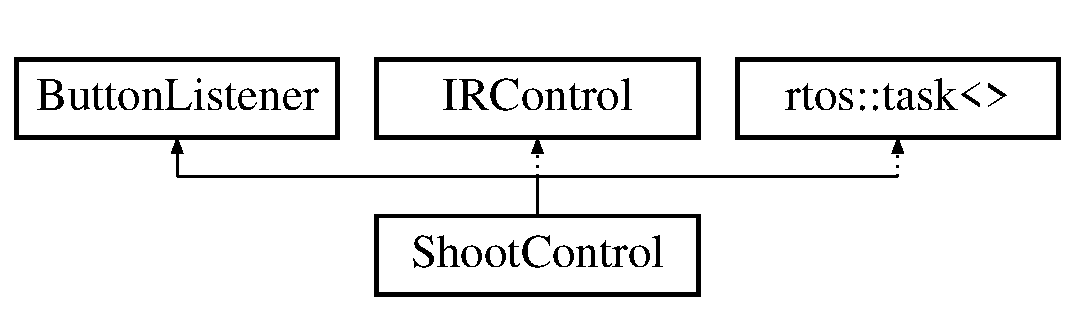
\includegraphics[height=2.000000cm]{class_shoot_control}
\end{center}
\end{figure}
\subsection*{Public Member Functions}
\begin{DoxyCompactItemize}
\item 
\mbox{\hyperlink{class_shoot_control_af9c21b16c798f217b2da762d569473cd}{Shoot\+Control}} (const char $\ast$name, int priority, \mbox{\hyperlink{class_i_r_control}{I\+R\+Control}} \&I\+R\+\_\+control, \mbox{\hyperlink{class_player_data}{Player\+Data}} \&player\+\_\+data, \mbox{\hyperlink{class_weapon}{Weapon}} \&weapon, hwlib\+::pin\+\_\+out \&laser\+\_\+pin)
\begin{DoxyCompactList}\small\item\em This is the constructor for the shoot\+Control. \end{DoxyCompactList}\item 
\mbox{\Hypertarget{class_shoot_control_a17f6db4ed8fb3a7195e03eb54b9c26f1}\label{class_shoot_control_a17f6db4ed8fb3a7195e03eb54b9c26f1}} 
void \mbox{\hyperlink{class_shoot_control_a17f6db4ed8fb3a7195e03eb54b9c26f1}{shoot}} ()
\begin{DoxyCompactList}\small\item\em This function sets the shoot\+\_\+flag.  This function is used to be called by another class. \end{DoxyCompactList}\item 
void \mbox{\hyperlink{class_shoot_control_afda9df061db3b34fdf9affed32f2c325}{main}} () override
\begin{DoxyCompactList}\small\item\em This function contains the state machine. \end{DoxyCompactList}\end{DoxyCompactItemize}


\subsection{Detailed Description}
This class encodes and sends the message to be sent to the \mbox{\hyperlink{class_i_r_control}{I\+R\+Control}} class and controls the laser. 

\subsection{Constructor \& Destructor Documentation}
\mbox{\Hypertarget{class_shoot_control_af9c21b16c798f217b2da762d569473cd}\label{class_shoot_control_af9c21b16c798f217b2da762d569473cd}} 
\index{Shoot\+Control@{Shoot\+Control}!Shoot\+Control@{Shoot\+Control}}
\index{Shoot\+Control@{Shoot\+Control}!Shoot\+Control@{Shoot\+Control}}
\subsubsection{\texorpdfstring{Shoot\+Control()}{ShootControl()}}
{\footnotesize\ttfamily Shoot\+Control\+::\+Shoot\+Control (\begin{DoxyParamCaption}\item[{const char $\ast$}]{name,  }\item[{int}]{priority,  }\item[{\mbox{\hyperlink{class_i_r_control}{I\+R\+Control}} \&}]{I\+R\+\_\+control,  }\item[{\mbox{\hyperlink{class_player_data}{Player\+Data}} \&}]{player\+\_\+data,  }\item[{\mbox{\hyperlink{class_weapon}{Weapon}} \&}]{weapon,  }\item[{hwlib\+::pin\+\_\+out \&}]{laser\+\_\+pin }\end{DoxyParamCaption})\hspace{0.3cm}{\ttfamily [inline]}}



This is the constructor for the shoot\+Control. 

The constructor expects the class \mbox{\hyperlink{class_i_r_control}{I\+R\+Control}} the enitities player\+\_\+data and weapon as well as a output pin for the laser. 

\subsection{Member Function Documentation}
\mbox{\Hypertarget{class_shoot_control_afda9df061db3b34fdf9affed32f2c325}\label{class_shoot_control_afda9df061db3b34fdf9affed32f2c325}} 
\index{Shoot\+Control@{Shoot\+Control}!main@{main}}
\index{main@{main}!Shoot\+Control@{Shoot\+Control}}
\subsubsection{\texorpdfstring{main()}{main()}}
{\footnotesize\ttfamily void Shoot\+Control\+::main (\begin{DoxyParamCaption}{ }\end{DoxyParamCaption})\hspace{0.3cm}{\ttfamily [inline]}, {\ttfamily [override]}}



This function contains the state machine. 

This function contains only one state called idle. The idle state waits for a shoot flag. When the shoot flag is set the laser turns on and the function set\+Send\+Data is called. After 100ms the laser is turned off and the state starts waiting for the shoot\+\_\+flag again. 

The documentation for this class was generated from the following file\+:\begin{DoxyCompactItemize}
\item 
C\+:/ti-\/software/thema\+\_\+opdracht\+\_\+lasergame/\+Player/\mbox{\hyperlink{_shoot_control_8hpp}{Shoot\+Control.\+hpp}}\end{DoxyCompactItemize}

%--- End generated contents ---

% Index
\backmatter
\newpage
\phantomsection
\clearemptydoublepage
\addcontentsline{toc}{chapter}{Index}
\printindex

\end{document}
